\PassOptionsToPackage{numbers}{natbib}
\documentclass{mnnit}
\usepackage{graphicx}
\usepackage{booktabs}
\usepackage{amsmath}
\usepackage{amssymb}
\usepackage{url}
\usepackage{tikz}
\usetikzlibrary{arrows.meta,positioning,shapes.geometric,calc}
\usepackage{pgfplots}
\pgfplotsset{compat=1.17}
\usepackage{xcolor}
\usepackage[most]{tcolorbox}
\usepackage{algpseudocode}
\newtcolorbox{livebox}[2]{enhanced, breakable,
  colback=#2!5, colframe=#2!45, colbacktitle=#2!16,
  coltitle=black, fonttitle=\bfseries\small, title={#1},
  fontupper=\small, boxrule=0.5pt, arc=1.2mm,
  left=2mm, right=2mm, top=1.2mm, bottom=1.2mm,
  before skip=10pt, after skip=10pt}
\emergencystretch=3em

% mnnit.cls uses pre-1995 float internals that break on modern kernels;
% use non-floating blocks with these caption helpers instead.
\makeatletter
\newcommand{\figcaption}[1]{\def\@captype{figure}\caption{#1}}
\newcommand{\tabcaption}[1]{\def\@captype{table}\caption{#1}}
\makeatother

\begin{document}
\title{Design and Development of an Agentic Retrieval-Augmented
Generation Framework for Automated Legal Case Analysis}
\author{Samudraneel Sarkar (20233249), Patil Sakshi (20233209),
        Nikhil Kumar (20233202), and Manpreet Kaur (20233180)}
\titleauthors{Samudraneel Sarkar (20233249)\\
              Patil Sakshi (20233209)\\
              Nikhil Kumar (20233202)\\
              Manpreet Kaur (20233180)}
\signames{Samudraneel Sarkar & 20233249\\
          Patil Sakshi & 20233209\\
          Nikhil Kumar & 20233202\\
          Manpreet Kaur & 20233180}
\submitdate{November 2026}
\supervisor{Dr.\ Vibhav Prakash Singh}

\specialization{Computer Science \& Engineering}
\beforepreface

\prefacesection{Abstract}
Automated analysis of legal cases to find applicable
judgements and precedents is a promising application of large
language models. However, in law, every claim or argument must
be traceable to an authoritative legal document and LLMs often
fall prey to hallucination and fabricated language generation.
We investigate how a retrieval augmented generation system
should be designed to handle legal work in realistic settings
where case descriptions run into several thousand tokens and
output must cite statutes and precedents that are directly
relevant. We quantitatively examine RAG pipelines and different
retrieval, embedding and chunking strategies and evaluate their
performances on the IL-PCSR benchmark, which evaluates Indian
statutes and case judgement precedents. We also validate
our findings on other Indian and international benchmarks, AILA
and BSARD, and establish three findings. First, the two retrieval tasks reward different
machinery: lexical retrieval dominates precedent finding,
whereas long context dense retrieval, often combined with
lexical retrieval by rank fusion, dominates statute retrieval.
Second, compression of any form of the case, including
expansion, rhetorical restriction, truncation for the
cross-encoder re-ranker, etc., degrades retrieval quality. Third, a re-ranker improves the ranking only
when relevant signal is semantic and the re-ranker can read the
complete query, and otherwise a truncated cross encoder leads
to worse performance. These findings produce an asymmetric
optimal architecture with a dense-lexical statute leg along
with language model reranking, and a purely lexical precedent
leg. We then test a bounded agent loop on top of this
pipeline to place guardrails like retry upon failure,
external fallback mechanism and mechanical validation of
citations, and evaluate the resulting architecture on an
expanded corpus of 28,074 section-level statute documents
covering 302 Central acts.

\prefacesection{Acknowledgements}
We express our sincere gratitude to our supervisor, Dr.\ Vibhav
Prakash Singh, Department of Computer Science and Engineering,
Motilal Nehru National Institute of Technology Allahabad, for his
guidance, help, and constructive feedback throughout this
project.

We also thank the faculty and staff of the Department of Computer
Science and Engineering for the environment and the resources
that made this work possible. We also thank the authors of the
IL-PCSR, BSARD, AILA, and related corpora for their invaluable
contributions in
releasing the datasets with reproducible baselines, without
which a fair comparative study could not have been conducted.
We also sincerely thank our friends at NUJS Kolkata for their
inputs on matters which require a legal perspective.

Finally, we thank our families and friends for their constant
support and love during the course of this work.

\afterpreface

\chapter{Introduction}

\section{Background}

The documents a legal system produces fall into two broad
classes. Statutes are acts of the legislature: prescriptive
texts organised hierarchically into chapters, sections, and
sub-sections, each section stating a rule, a definition, an
offence, or a remedy in compact formal language. The Indian
penal code, its successor the Bharatiya Nyaya Sanhita, and the
procedural and evidence codes are examples. Case law is the
second class: a judgment records the facts of a dispute, the
issues framed, the reasoning of the court, the ratio decidendi
that binds future courts, and the final order.

Large language models are neural networks trained to predict
the next token over very large text corpora. Their fluency comes
from parametric memory: the facts a model knows are encoded
implicitly in its weights rather than stored in any document it
can point back to, and the model will produce a plausible
continuation whether or not the underlying fact is true. Two
consequences matter for law. First, hallucination: a model can
emit a confident but non-existent section number or case
citation. Second, the context window: a model can only attend to
a bounded span of text, which a long judgment or a detailed case
description can exceed.

Applications of these models to law now span judgment
summarisation, document drafting, question answering, and
retrieval, and dedicated benchmarks measure them: LegalBench
collects a broad suite of legal reasoning
tasks~\cite{legalbench} and IL-TUR covers Indian legal text
specifically~\cite{iltur}. Long-input encoders such as
LawFormer extend the context budget for legal
documents~\cite{lawformer}, while specialised encoders such as
SAILER are trained for case retrieval~\cite{sailer}. What these
applications share is a dependence on retrieval: the answer a
legal system gives is only as trustworthy as the documents it
was built from, which is the central concern of this study.

\section{Motivation}
India administers one of the largest judicial systems in the
world. The National Judicial Data Grid records tens of millions
of pending matters across the district and subordinate
courts~\cite{njdg}, and behind each matter lies a recurring
research task: given a set of facts, identify the statutory
provisions that govern it and the prior judgments that bear upon
it. Legal professionals perform this task against a corpus that
is large, formally phrased, and constantly amended; a single case
description can run to several thousand tokens before a single
authority is consulted. Any reduction in the effort required to
locate and verify the applicable law has direct practical value.

Large language models attend to this need. However, they operate
like black boxes, and therefore their results cannot be verified
easily. A model asked for the punishment for murder can produce
a confident section number or a confident precedent name.
However, there is no mechanism by which a reader can distinguish
a true citation from a plausible fabrication or hallucination.

Retrieval-augmented generation supplies the grounding
mechanism~\cite{rag}. Whether it suffices for legal case
analysis is, however, an empirical question rather than an
assumption. The queries are not keyword strings but complete
case descriptions averaging roughly 4,500 tokens; the corpora are
of two kinds whose notions of relevance differ; and the retrieval
machinery deployed in most RAG systems is designed and validated
for short queries. Which components of that machinery transfer to
long legal queries, which do not, and what an agentic controller
contributes beyond a fixed pipeline, are the questions this
dissertation answers through controlled measurement followed by
system construction.

A property of the reported literature narrows the design space
further. For the benchmarks most relevant to this task, the
strongest published rows are produced by systems fitted to the
benchmark itself: the leading IL-PCSR configuration trains a
graph network on corpus-specific rhetorical labels, and the
leading BSARD rows are fine-tuned bi-encoders (Sections~3.12
and~3.13). The legal corpus is not a fixed index, however.
Courts deliver judgments and legislatures enact, amend, and
repeal provisions continually, so a fitted component begins to
drift the day it is trained, and a production system cannot
re-fine-tune on a schedule the corpus does not keep. This
dissertation therefore treats benchmark-specific training as
the exception rather than the method: the target is a
configuration assembled from training-free legs that remains
competitive with the published rows and transfers to new
corpora without modification.

\section{Problem Statement}
The task is automated legal case analysis over Indian law,
formalised as follows.

\medskip
\noindent\textbf{Input.} A natural-language case description $q$
of several thousand tokens, comprising a factual narrative, the
issues framed, and the procedural history of the matter, in the
form used by the IL-PCSR benchmark~\cite{ilpcsr}.

\medskip
\noindent\textbf{Output.} Three artefacts: (i) an ordered set $S$
of statutory provisions drawn from a statute corpus, (ii) an
ordered set $P$ of precedent documents drawn from a precedent
corpus, and (iii) a structured dossier $D$ containing a direct
answer, the applicable provisions, a grounded analysis, and
recommended steps, such that every substantive claim in $D$ is
supported by an element of $S \cup P$ and carries a verifiable
citation.

\medskip
\noindent\textbf{Functional requirements.}
\begin{description}
\item[R1 Grounding.] Every emitted claim must cite a document
  present in the retrieved evidence set; unverifiable identifiers
  are suppressed mechanically. When retrieval cannot supply
  adequate evidence, the system must disclose the insufficiency
  and invoke an external fallback rather than present ungrounded
  material as retrieved authority.
\item[R2 Sufficiency awareness.] The system must determine
  whether the retrieved evidence genuinely addresses the case,
  independently of retrieval scores, which cannot distinguish a
  correct statute from a lexically similar incorrect one.
\item[R3 Bounded recovery.] Insufficient evidence must trigger a
  bounded re-retrieval, and persistent insufficiency must route
  to an external source explicitly labelled as not
  corpus-grounded.
\end{description}

\medskip
The problem is difficult for three reasons. First, the input is
long: an IL-PCSR case description averages roughly 3,600 words,
which exceeds the input budget of standard embedding models and
cross-encoders, so part of the information need is invisible to
them by construction. Second, the two output corpora embody
different notions of relevance: statutes are relevant
doctrinally, by mapping facts to the elements of a provision,
whereas precedents are relevant factually, by similarity of
situation and vocabulary. There is no reason to expect a single
retriever to be optimal for both. Third, the correctness
constraint is strict: a system that emits a plausible but
incorrect citation has failed materially, not marginally.

\section{Research Objectives}
\begin{enumerate}
\item To establish, through controlled experiments on a public
  Indian legal benchmark, which retrieval, fusion, reranking, and
  query-processing mechanisms are effective for long-form statute
  and precedent retrieval.
\item To derive from those measurements a retrieval architecture
  in which each component is justified by evidence rather than by
  convention.
\item To design an agentic control loop that adds to the fixed
  pipeline the guarantees it lacks: evidence-sufficiency
  judgment, bounded recovery, citation validation, and labelled
  external assistance.
\item To implement the framework as a working application over an
  expanded Indian statutory corpus, and to verify its behaviour
  on queries the benchmark itself cannot answer.
\item To examine whether the derived architecture and its design
  rules transfer to other legal datasets and jurisdictions.
\end{enumerate}

\section{Scope of the Study}
The study addresses retrieval and grounded synthesis for Indian
central legislation and case law in English. It does not attempt
legal judgment prediction, statutory interpretation as a
normative exercise, drafting of legal instruments, or
jurisdictions outside India. Benchmark evaluation is conducted on
the IL-PCSR development split; the published test-split figures
of the benchmark are cited under their own protocol and are not
equated with development-split figures. Language-model calls in
the system use externally hosted models.

\chapter{Literature Review and Theoretical Foundations}

\section{Legal Informatics and the Case Analysis Problem}
Computational assistance for legal research predates neural
methods. Early systems relied on the vector space
model~\cite{salton1975vector} and on term-weighting
schemes~\cite{salton1988termweight}; the probabilistic framework
that succeeded them produced BM25~\cite{bm25}, which remains the
standard lexical baseline decades later. Two properties of legal
text shaped this line of work: legal meaning is carried by
phrases rather than isolated terms, and the documents are long.
Statute identification in particular has been approached through
multi-label classification~\cite{luo2017fla,zhong2018topjudge}
and through graph-based methods such as LeSICiN, which models
statute hierarchy for Indian
documents~\cite{paul2022ilsi,paul2024legal}. Prior case retrieval
has been modelled as ranking from the outset, because the
candidate pool is large and relevance is
similarity-based~\cite{feng2024pcrsurvey}.

Indian legal text presents a specific structural property on
which part of this study depends: judgments are not segmented
into facts, issues, arguments, and rulings by any reliable
marker. The rhetorical-role literature supplies automatic
segmentation instead. The ILDC corpus established sentence-level
legal segmentation for Indian judgments~\cite{malik2021ildc};
Malik et al.\ labelled rhetorical roles such as Facts, Issue, and
Court Reasoning~\cite{malik2022rr}; and DeepRhole provides a
trained classifier for the same
labels~\cite{bhattacharya2023deeprhole}. The IL-PCSR queries used
in this study carry exactly these segment annotations, which
makes a rhetorical-restriction ablation directly executable.

\section{Language Models and the Verifiability Problem in Law}
Large language models have been evaluated across legal tasks by
LegalBench~\cite{legalbench} and, for Indian law specifically, by
IL-TUR~\cite{iltur}. A consistent finding across this literature
is that model fluency is not accompanied by source fidelity:
models produce provisions and case names that read correctly and
do not exist. Domain adaptation has been attempted through
pretraining on legal corpora; SAILER trains a structure-aware
encoder for case retrieval~\cite{sailer}, and LawFormer extends
the input budget for long legal documents~\cite{lawformer}. The
present study measures rather than assumes the benefit of such
models on the task at hand, and its results for unmodified
legal-domain encoders are negative.

\section{Retrieval-Augmented Generation}
Retrieval-augmented generation conditions a generated answer on
documents retrieved at inference time~\cite{rag}. The
architecture transfers the burden of factuality from the
generator's parametric memory to the retriever's index, which is
auditable. Its performance is therefore bounded by retrieval
quality, and the design space of that retriever is the subject of
the next three sections.

\section{First-Stage Retrieval}
\subsection{Lexical Retrieval}
BM25 scores a document against a query by
inverse-document-frequency-weighted term overlap, with
term-frequency saturation and document-length
normalisation~\cite{bm25}. Three of its properties matter to this
task. It is deterministic, so its rankings are fully auditable.
It rewards phrase overlap when indexed over word $n$-grams, which
matches how statutory and judicial language encodes meaning.
Its cost does not grow with query length, since additional query
terms only refine the match. The implementation decision that
dominates its behaviour on legal text is the tokenisation unit:
word $n$-grams preserve multi-word terms of art such as
\emph{culpable homicide} or \emph{unlawful assembly} that unigram
indexing fragments~\cite{bm25s}.

\subsection{Dense Retrieval}
Dense retrievers map queries and documents into a shared vector
space with a bi-encoder and rank by
similarity~\cite{dpr,sbert}. Their advantage is semantic
generalisation: a document can be retrieved without sharing any
vocabulary with the query. The corresponding risk is that the
match is not phrase-verifiable, and two constraints govern their
use on this task. The first is context length: a 512-token
encoder reads roughly a seventh of an average IL-PCSR case
description and ranks on that fragment alone, while longer-input
models such as the Qwen3-Embedding
family~\cite{qwen3emb} read several times as much. The second is
task fit: a legal-domain encoder pretrained for one retrieval
objective does not automatically transfer to the matching of case
descriptions to provisions.

\subsection{Hybrid Retrieval and Fusion}
Lexical and dense retrievers fail in complementary ways, which
motivates fusion. Reciprocal rank fusion combines ranked lists by
position alone, assigning each document
$\sum_{r} 1/(k + \mathrm{rank}_r)$ over the contributing
retrievers~\cite{rrf}. The method requires no score calibration,
but it interpolates rather than amplifies: fusing a strong leg
with a weak leg produces a ranking between the
two~\cite{bruch2023fusionhybrid}. Whether this interpolation
helps or harms depends on whether both legs carry signal, which
Chapter 3 measures per task.

\subsection{Second-Stage Reranking}
A reranker rescores a small candidate pool with a more expensive
model. Cross-encoders score each query-document pair
jointly~\cite{monobert}; late-interaction models preserve
token-level alignment~\cite{colbert}; learned sparse
representations combine lexical and neural
views~\cite{splade,bgem3}; and listwise methods ask a generative
model to order the pool directly, an approach whose effect on
legal ranking has been measured separately by Ma et
al.~\cite{ma2024llmrelevance} and by the IL-PCSR baseline
itself~\cite{ilpcsr}. All of these share one constraint that
decides their behaviour on this task: a reranker that cannot read
the full query cannot rank against it.

\section{Query Processing}
The standard interventions on a query are expansion, restriction,
reformulation, and truncation. Pseudo-relevance feedback expands
the query with terms harvested from the first-pass
results~\cite{rocchio}; on a corpus whose queries are already
long and redundant, its benefit is questionable by inspection and
is measured here directly. Restriction keeps only selected
rhetorical-role segments, an application of the segmentation
literature~\cite{malik2022rr,bhattacharya2023deeprhole} to
retrieval rather than to labelling. Reformulation and
summarisation compress the query, the strategy the IL-PCSR
baseline itself employs for its summary-conditioned
models~\cite{ilpcsr}. Truncation is the implicit intervention of
every bounded-context model. Chapter 3 evaluates each.

\section{Agentic Workflows}
An agentic system places a language model in the control loop:
the model selects tools, inspects intermediate results, and
iterates~\cite{react,agenticrag}. Self-reflective retrieval goes
further and has the model explicitly assess whether retrieved
evidence suffices before generating~\cite{selfrag}. For legal
case analysis the candidate agentic contributions are four: a
judgment of evidence sufficiency that lexical scores cannot
supply, one reformulated retrieval upon failure, a graceful and
labelled fallback when the corpus lacks the answer, and
mechanical verification that emitted citations exist in the
retrieved set. Prior case retrieval research has used event
extraction~\cite{joshi2023ucreat}, graph neural
networks~\cite{tang2024casegnn,tang2024caselink}, citation
structure~\cite{bhattacharya2020hierspcnet}, and judgment-guided
retrieval~\cite{qin2024ljpretrieval}; the IL-PCSR benchmark ties
several of these threads together and supplies the evaluation
bed for this study~\cite{ilpcsr}.

\section{Research Gaps}
Three gaps follow from the literature. First, published legal
retrieval evaluations compare retrievers on uniform settings, but
the two legal corpora reward different notions of relevance;
whether legs should differ per task is measured here rather than
assumed. Second, standard query-processing interventions are
evaluated for short queries; their behaviour on multi-thousand
token case descriptions is an open question with a uniform
answer. Third, agentic RAG systems are described qualitatively in
the literature; their measurable contribution over a fixed
pipeline on a shared benchmark, including citation validity
rates, is not. This dissertation addresses all three.

\chapter{Methodology and Experimental Investigation}

\section{The IL-PCSR Benchmark}
IL-PCSR~\cite{ilpcsr} is a parallel corpus for statute and
precedent retrieval over Indian case judgments. It comprises
6,271 expert-labelled case descriptions partitioned into 5,017
training, 627 development, and 627 test queries. Each query is a
complete judgment segmented into rhetorical-role
spans~\cite{malik2022rr,kalamkar2022corpus}, averaging roughly
3,600 words and 40 segments on the development split, with
explicit statute and precedent citations masked by the dataset
authors using a legal named-entity recogniser and personal names
anonymised for bias control~\cite{kalamkar2022legalner}.

The two gold corpora differ in nature. The statute pool contains
936 documents, sections drawn from central acts, averaging about
716 words each; the precedent pool contains 3,183 judgments of
the Supreme Court and the High Courts, averaging about 7,900
words each. Development queries cite 3.73 statutes and 2.72
precedents on average.

The two retrieval tasks differ fundamentally. Statute retrieval
(LSR) requires mapping factual circumstances to governing
provisions; the relevance signal is doctrinal. Precedent
retrieval (PCR) requires identifying prior cases of similar
situation; the relevance signal is factual similarity, expressed
largely in shared phrases and procedural context. The experiments
in this chapter repeatedly turn on this distinction.

\section{Task Formalisation}
Given a query $q$ and a candidate pool $\{c_1,\dots,c_l\}$, with
$c_i \in \mathcal{S}$ for LSR and $c_i \in \mathcal{P}$ for PCR,
a retrieval model produces a ranked list
$\hat{C}(q) = [c_{q_1}, \dots, c_{q_l}]$ by decreasing relevance
score. The gold set for $q$ is the set of candidates actually
cited by the judgment, with citation strings masked from the
query text. The output consumed downstream is the top-$k$ prefix
of $\hat{C}(q)$.

\section{Metrics and Evaluation Protocol}
Retrieval quality is reported as recall@$k$, precision@$k$,
macro-F1@$k$, mean average precision (MAP), mean reciprocal rank
(MRR), and nDCG@$k$, computed per query and macro-averaged. All
experiments in this chapter evaluate the development split at
$k=10$ unless stated otherwise; the agent benchmark uses a
50-query development slice at $k=8$.

Two protocol distinctions are stated once and then used
throughout. The published IL-PCSR table reports macro-F1 at the
best per-query depth on the test split, an oracle over evaluation
depths; this study reports fixed-depth F1@10 on the development
split. The two protocols are not numerically equivalent:
comparisons are therefore stated in terms of which mechanism
dominates inside each protocol, never in terms of raw numbers.

\section{The Experiment Harness}
All configurations execute through a shared harness. A JSON
specification declares the dataset slice, chunking strategy,
retriever, query strategy, and reranker; the runner builds or
loads the index, issues every query through an identical code
path, and writes per-query metric files, and each run records its
git commit, config hash, seed, and platform in the result file.
Compute-bound legs (dense encoding, cross-encoder reranking, and
listwise reranking) executed on remote GPU infrastructure, a
Kaggle T4 for lighter workloads and a Modal A10G for heavier
ones; lexical experiments ran on CPU. The harness's BM25 leg uses
BM25S over word $n$-grams with $k_1=1.6$ and $b=0.7$~\cite{bm25s}.

\section{Experimental Design}
The investigation proceeds as a sequence of questions, each
answered by a named configuration.

\noindent\textbf{Experiment 1: tokenisation and granularity.}
Whole-document unigram BM25 against $n$-gram variants and chunked
indexing, establishing the lexical baseline and the effect of
document segmentation.

\noindent\textbf{Experiment 2: dense first-stage retrieval.}
General-purpose embedders (BGE), legal-domain embedders
(Legal-Embed, SAILER), and long-context embedders
(Qwen3-Embedding-0.6B and 4B), under the context budgets their
models impose.

\noindent\textbf{Experiment 3: rank fusion.} Reciprocal rank
fusion ($k=60$) over lexical-dense pairs, on both tasks, testing
whether fusion helps where constituent legs are and are not
competitive.

\noindent\textbf{Experiment 4: second-stage reranking.} A
cross-encoder (bge-reranker-v2-m3, 2,048-token window) and a
listwise language-model reranker (a reasoning model over the
fused top-50 pool, 20 numbered snippets of 1,000 characters
each), against their first-stage pools.

\noindent\textbf{Experiment 5: query processing.}
Pseudo-relevance feedback at three settings, restriction to
rhetorical-role segments in four configurations, and the
truncation and reformulation effects observable across the other
experiments.

\noindent\textbf{Experiment 6: the agentic loop.} A 50-query
benchmark of the route-retrieve-reflect-synthesise agent,
measuring retrieval quality of its final evidence union alongside
its behavioural statistics.

\noindent\textbf{Experiment 7: learned sparse and late
interaction.} BGE-M3 in all four of its modes: dense, learned
sparse, RRF union, and ColBERT MaxSim rerank over the union pool.

\section{First-Stage Results}
Table~\ref{tab:firststage} reports the first-stage
configurations.

\begin{center}
\small
\tabcaption{First-stage retrieval on the development split
($n=627$). Best per column in bold; the 5-gram precedent row was
measured on the whole-document index required by that
tokenisation.}
\label{tab:firststage}
\vspace{2mm}
\begin{tabular}{lccccc}
\toprule
 & \multicolumn{3}{c}{Statute (LSR)} & \multicolumn{2}{c}{Precedent (PCR)} \\
\cmidrule(lr){2-4}\cmidrule(lr){5-6}
Configuration & F1@10 & MAP & MRR & F1@10 & MAP \\
\midrule
BM25 unigram, whole document & 8.39 & 9.57 & 20.55 & 11.02 & 18.41 \\
BM25, fixed-512 chunks & 11.61 & 12.90 & 28.92 & 16.48 & 19.11 \\
BM25, recursive-512 chunks & 11.46 & 12.87 & 29.38 & 17.19 & 19.75 \\
BM25 2-gram, recursive-512 & 10.55 & 12.59 & 30.77 & 20.15 & 27.11 \\
BM25 5-gram, whole document & --- & --- & --- & \textbf{20.73} & \textbf{39.90} \\
BGE-base, 512-token & 5.67 & 6.72 & 14.73 & 4.05 & 5.73 \\
Legal-Embed & 7.98 & 9.01 & 19.35 & 4.34 & 6.74 \\
SAILER & 0.23 & 0.12 & 0.47 & 0.02 & 0.04 \\
Qwen3-Embedding-0.6B & 12.57 & 15.16 & 30.93 & 11.07 & 17.18 \\
Qwen3-Embedding-4B & \textbf{14.29} & \textbf{19.79} & 37.38 & 12.59 & 19.65 \\
\bottomrule
\end{tabular}
\end{center}

The two tasks exhibit opposite preferences. On precedents the
parameter-free lexical leg dominates outright: whole-document
5-gram BM25 approximately doubles the MAP of the best dense
configuration, because precedent relevance in this benchmark is
factual similarity and factual similarity is carried by shared
phrases that $n$-gram matching reads directly. On statutes the
ordering inverts: lexical retrieval is weak, the long-context
embedders are strong, and the 4B variant is the strongest single
leg measured. The same evaluation ranking dense retrieval last on
one task and first on the other is the direct argument for
task-conditional legs.

Three subsidiary results are instructive. Every 512-token
embedder scores below even chunked BM25 on both tasks, because it
ranks documents against a fraction of the query. SAILER, a
legal-domain encoder, scores near zero on both tasks, indicating
that pretraining on legal text does not imply competence at this
matching task. And chunk granularity is a second-order decision:
recursive-512 and fixed-512 differ within noise, while
whole-document indexing wins where $n$-gram phrase context must
span the document.

\section{Fusion Results}
Table~\ref{tab:fusion} reports reciprocal rank fusion over the
first-stage legs.

\begin{center}
\small
\tabcaption{Reciprocal rank fusion on the development split. The
fused pool is formed from each leg's top ranks at $k=60$.}
\label{tab:fusion}
\vspace{2mm}
\begin{tabular}{lccccc}
\toprule
 & \multicolumn{3}{c}{Statute (LSR)} & \multicolumn{2}{c}{Precedent (PCR)} \\
\cmidrule(lr){2-4}\cmidrule(lr){5-6}
Configuration & F1@10 & MAP & MRR & F1@10 & MAP \\
\midrule
RRF: BM25 + BGE-base & 8.29 & 9.48 & 19.97 & 10.09 & 15.35 \\
RRF: 5-gram BM25 + Qwen3-0.6B & 13.65 & 17.91 & 38.91 & 19.09 & 29.85 \\
RRF: 5-gram BM25 + Qwen3-4B & \textbf{14.68} & \textbf{19.12} & \textbf{40.53} & 19.74 & 31.60 \\
\bottomrule
\end{tabular}
\end{center}

Fusion improves retrieval precisely where the constituent legs
are competitive. On statutes, fusing the lexical and long-context
dense legs produces the strongest first-stage ranking measured,
exceeding either leg alone, because the legs err in different
places and both carry signal. On precedents the same operation
draws the dominant lexical ranking toward the weaker dense one
and loses ground relative to 5-gram BM25 alone; fusing BM25 with
the weak BGE leg degrades statutes as well. The pattern is
consistent: fusion interpolates rankings rather than creating
signal, so its benefit is conditional on leg quality, not
automatic.

\section{Reranking Results}
Table~\ref{tab:rerank} reports the two second stages against
their first-stage pool.

\begin{center}
\small
\tabcaption{Second-stage reranking over the fused top-50 pool.
The listwise reranker reads the query (up to 4,000 characters)
beside 20 numbered snippets.}
\label{tab:rerank}
\vspace{2mm}
\begin{tabular}{lccccc}
\toprule
 & \multicolumn{3}{c}{Statute (LSR)} & \multicolumn{2}{c}{Precedent (PCR)} \\
\cmidrule(lr){2-4}\cmidrule(lr){5-6}
Configuration & F1@10 & MAP & MRR & F1@10 & MAP \\
\midrule
First-stage pool (RRF c2) & 13.65 & 17.91 & 38.91 & 19.09 & 29.85 \\
Cross-encoder rerank & 7.46 & 6.56 & 16.14 & 6.89 & 7.28 \\
LLM listwise rerank & \textbf{14.83} & \textbf{25.20} & \textbf{50.88} & 16.62 & 25.48 \\
\bottomrule
\end{tabular}
\end{center}

The cross-encoder result is the clearest context-length failure
in the study. Truncated to 2,048 tokens, it scores candidates
against roughly the first half of each case description and draws
both tasks below their first-stage pools; precedent recall@10
collapses from 53.1\% to 19.2\%, so the ordering it emits is
anti-correlated with relevance rather than merely weak. The
failure is of context, not of ranking quality: a second stage
that cannot read the query ranks a different problem from the one
posed.

The listwise reranker shows the mirror image. Because the
language model reads enough of the query alongside the
candidates, it improves the statute leg substantially, gaining
7.3 MAP points and 12.0 MRR points over its pool and reaching a
best-depth F1 of 23.8 at $k{=}2$. The same operation reduces
precedent MAP by 4.5 points, consistent with the task's
phrase-lexical relevance signal being invisible to semantic
judgment. Reranking is therefore included on the statute leg and
excluded from the precedent leg, each for measured reasons.

\section{Query-Processing Results}
Four interventions, each a defensible attempt to improve a long
query, all degraded retrieval (Table~\ref{tab:query}).

\begin{center}
\small
\tabcaption{Query-processing interventions. Reference rows are
the unmodified-query runs on the same index; the PRF statute row
scores 6.85 F1@10 against a 10.55 reference.}
\label{tab:query}
\vspace{2mm}
\begin{tabular}{lcc}
\toprule
Intervention & F1@10 & MAP \\
\midrule
\multicolumn{3}{l}{\emph{Precedent task (5-gram BM25, filtered index)}} \\
Full query (reference) & 20.73 & 39.90 \\
PRF expansion ($d{=}3,e{=}10$) & 19.15 & 32.49 \\
Facts + Issue segments only & 3.86 & 5.21 \\
Facts segments only & 5.93 & 9.11 \\
Issue segments only & 3.73 & 5.91 \\
All segments except Court Reasoning & 18.05 & 31.55 \\
\midrule
\multicolumn{3}{l}{\emph{Statute task (2-gram BM25)}} \\
Facts + Issue segments only & 4.63 & 5.04 \\
All segments except Court Reasoning & 7.41 & 9.56 \\
\bottomrule
\end{tabular}
\end{center}

Pseudo-relevance feedback drifts the query toward whatever the
first pass already retrieved, including its errors, and the
deviation is near zero across all three expansion settings.
Restricting the query to individual rhetorical sections
collapses retrieval almost entirely, because the procedural
posture and reasoning context carry signal that no single
section holds. Removing only the Court Reasoning segments costs
about eight MAP points on precedents and is mildly harmful on
statutes as well. Truncation was examined in Section~3.8, and
reformulation inside the agent benchmark loses the specific
vocabulary the gold documents employ. Each mechanism fails
differently, and all fail; the serving pipeline consequently
issues the case text verbatim.

\section{Agent Benchmark Results}
The 50-query agent benchmark exercises the full loop
(Table~\ref{tab:agent}).

\begin{center}
\small
\tabcaption{Agent benchmark, 50-query development slice, BM25
2-gram legs at top-8.}
\label{tab:agent}
\vspace{2mm}
\begin{tabular}{lr}
\toprule
Quantity & Value \\
\midrule
Queries evaluated & 50 \\
Retrieval calls issued & 78 \\
First verdict: evidence sufficient & 22 \\
Complete dossiers produced & 49 of 50 \\
Citations emitted & 167 \\
Citations failing validation & 0 \\
Total LLM latency & 830.9 s \\
Wall-clock duration & 13.9 min \\
\bottomrule
\end{tabular}
\end{center}

The call count exhibits the loop in operation: 28 of 50 queries
failed their first sufficiency verdict, were re-retrieved once
with reformulated queries, and all but one then produced a
complete dossier. The citation row states the property a legal
tool cannot compromise: no emitted citation required removal.
The retrieval-quality side is equally instructive: the agent's
evidence union scores below the verbatim single-shot arm
(statute MAP 9.5 against 12.6; precedent 7.0 against 27.1),
because the router's shortened queries lose the vocabulary that
drives lexical retrieval.

\section{Learned Sparse and Late-Interaction Results}
BGE-M3 was evaluated in all four of its modes on both tasks
(Table~\ref{tab:bgem3}).

\begin{center}
\small
\tabcaption{BGE-M3 all-modes on the development split. All four
modes score below the corresponding lexical or Qwen3 legs.}
\label{tab:bgem3}
\vspace{2mm}
\begin{tabular}{lccccc}
\toprule
 & \multicolumn{3}{c}{Statute (LSR)} & \multicolumn{2}{c}{Precedent (PCR)} \\
\cmidrule(lr){2-4}\cmidrule(lr){5-6}
BGE-M3 mode & F1@10 & MAP & MRR & F1@10 & MAP \\
\midrule
Dense & 7.76 & 9.24 & 19.94 & 9.53 & 14.68 \\
Learned sparse & 10.23 & 12.32 & 24.84 & 11.07 & 17.05 \\
RRF union & 7.84 & 6.04 & 13.46 & 12.02 & 18.40 \\
ColBERT MaxSim rerank & 6.82 & 8.49 & 18.50 & 8.21 & 11.75 \\
\bottomrule
\end{tabular}
\end{center}

No mode approaches the task champions: the strongest BGE-M3
configuration trails 5-gram BM25 on precedents by roughly twenty
MAP points and trails the fused Qwen3 leg on statutes. The
late-interaction reranker, which the published baseline does not
evaluate, performs worst of all, a second data point for the
context-length constraint that governs this task family.

\section{Comparison with the Published Baseline}
The published IL-PCSR table reports, on the test split under the
best-$k$ protocol, whole-document 5-gram BM25 as the strongest
lexical row and GPT-4.1 two-stage reranking over a fine-tuned
ensemble as the strongest configuration evaluated~\cite{ilpcsr}.
The strongest non-fine-tuned mechanism in that table is the same
class this study ranks strongest on the development split, and
the strongest reranker class agrees as well. The differences
beyond that shared base are the task-conditional legs, the
agentic loop, and the expanded corpus.

\begin{center}
\footnotesize
\setlength{\tabcolsep}{4pt}
\tabcaption{IL-PCSR rows against the assembled legs. Every block
reports the best per-configuration depth; IL-PCSR rows measure
the test split, this work the development split.}
\label{tab:baseline}
\vspace{2mm}
\begin{tabular}{ll ccc ccc}
\toprule
 & & \multicolumn{3}{c}{Statute (LSR)} & \multicolumn{3}{c}{Precedent (PCR)} \\
\cmidrule(lr){3-5}\cmidrule(lr){6-8}
System & Training & F1 & MAP & MRR & F1 & MAP & MRR \\
\midrule
\multicolumn{8}{l}{\emph{IL-PCSR, no training (test split, best-$k$)}}\\
BM25 para-wise, Max-All & none & 18.59 & 21.82 & 44.32 & 27.87 & 38.15 & 52.32 \\
BM25 5-gram, full doc. & none & 16.98 & 17.88 & 40.08 & 33.29 & 43.98 & 58.55 \\
\midrule
\multicolumn{8}{l}{\emph{This work, no training (dev split, best-$k$)}}\\
\textbf{RRF + Qwen3 + LLM rerank} & \textbf{none} & \textbf{23.82} & \textbf{25.20} & \textbf{50.88} & 19.28 & 25.48 & 39.23 \\
\textbf{BM25 5-gram, whole doc.} & \textbf{none} & --- & --- & --- & \textbf{32.19} & \textbf{39.90} & \textbf{57.28} \\
\midrule
\multicolumn{8}{l}{\emph{IL-PCSR, trained on benchmark (test split, best-$k$)}}\\
Para-GNN + BM25 ensemble & fine-tuned & 39.44 & 52.13 & 73.77 & 38.77 & 50.21 & 63.81 \\
\quad + GPT-4.1 rerank, 2-stage & + API & 46.11 & 61.06 & 81.55 & 43.31 & 54.43 & 68.88 \\
\bottomrule
\end{tabular}
\end{center}

Within the training-free tier the assembled statute leg leads on
every metric: F1 23.82 at its best depth against 18.59 for the
strongest published lexical row, MAP 25.20 against 21.82, and
MRR 50.88 against 44.32. The precedent leg sits within roughly a
point of the published 5-gram row on all three metrics (32.19,
39.90, 57.28 against 33.29, 43.98, 58.55), the residual expected
between development and test splits. The upper rows of the
published table, however, share a property the lower rows do
not: they are trained on the benchmark itself.

Para-GNN requires rhetorical-role labels for every paragraph,
which the benchmark obtains from the source website's
annotations, a corpus-specific resource; a per-document graph
linking paragraph nodes to a global node through role-labelled
edges; and a two-layer graph attention network trained
contrastively for one hundred epochs with one positive and 999
negatives per query on an 80\,GB accelerator, all of it
conditioned on labelled query--candidate pairs for the corpus in
question. The ensemble adds a further fitted component, a
per-query fusion weight learned by transfer between the two
tasks.

Nor is the headline row exempt: the GPT-4.1 figures are produced
by reranking the candidate pool of that fine-tuned ensemble, so
the strongest published stack depends end to end on trained
components.

A live legal corpus invalidates this arrangement. Judgments are
delivered and statutes are enacted, amended, or repealed
continuously, and each expansion of jurisdiction introduces
fresh statute families; every such addition obliges
re-segmentation, re-graphing, and eventually re-fitting on new
labels. At scales well beyond the benchmark's pools --- the
expanded statute corpus alone indexes 28,074 documents, against
936 in the benchmark --- and on text this syntactically and
semantically dense, periodic retraining is not a maintenance
task a practitioner can run. The framework therefore commits to
legs whose index updates are stateless and incremental: a new
document is tokenised or encoded, and no model is re-fitted.
For the ever-expanding corpora of ordinary legal work, the
training-free configuration is the appropriate design point,
and the accuracy headroom that supervision buys, quantified
under one protocol, is the first item of future work.

\section{External Validation}
The measurements so far describe a single benchmark. To test
whether the design rules travel, the pipeline is run unchanged
on two unrelated corpora: BSARD~\cite{louis2022bsard}, a Belgian
statutory benchmark authored in French, and AILA~\cite{aila}, an
Indian benchmark from the FIRE legal-assistance track.

\subsection{BSARD}
The statute leg is run on
BSARD~\cite{louis2022bsard}, a Belgian
statutory-article benchmark authored in French: 22,633 articles
and 222 jurist-labelled test questions, whose published
evaluation reports recall at depth~100 against a series of
zero-shot and fine-tuned baselines. The legs, metrics, and
protocol of this chapter are applied verbatim; the corpus
requires no code change beyond document loading, and no model is
trained.

Three observations follow (Table~\ref{tab:bsard}). First, the
n-gram ordering inverts as the framework predicts. BSARD
questions are legal questions of a dozen tokens rather than
multi-thousand-token case descriptions, so phrase n-grams starve:
the 5-gram configuration that leads precedent retrieval on
IL-PCSR collapses to 0.83 F1, while the unigram lexical leg and
the dense leg compete on near-equal terms. The rules are
query-conditional, not corpus-bound. Second, the measured
mechanisms transfer individually: prepending the act-context
description to indexed article text, the same device that
resolved act-name ambiguity in the expanded corpus, lifts
unigram MAP from 13.20 to 15.14, and reciprocal rank fusion over
the lexical and dense legs lifts recall at depth~100 from 51.65
to 54.62. Third, the assembled configuration exceeds every
zero-shot baseline published for the benchmark, including its
best dense bi-encoder row at 49.41 and its own BM25 row at
40.13; only the fine-tuned models score higher, at 74.78,
reproducing the supervision headroom observed on IL-PCSR. The
published rows are macro-averaged over queries while ours are
micro-averaged, a mild protocol difference that changes no
ranking here.

\begin{center}
\small
\tabcaption{External validation on BSARD (222 test questions,
22,633 French articles). This work reports micro-averaged
metrics at depth~100; published rows report the paper's
macro-averaged R@100.}
\label{tab:bsard}
\vspace{2mm}
\begin{tabular}{lcccc}
\toprule
Configuration & R@10 & R@100 & MAP@100 & MRR@100 \\
\midrule
BM25, unigram, context-prepend & 14.81 & 41.23 & 17.31 & 25.73 \\
Qwen3-Embedding-0.6B & 22.71 & 51.65 & 26.71 & 39.35 \\
Qwen3-Embedding-4B & 29.59 & \textbf{67.67} & \textbf{36.91} & \textbf{51.20} \\
RRF, BM25 + Qwen3-0.6B ($k{=}60$) & 22.08 & 54.62 & 25.88 & 37.62 \\
RRF, BM25 + Qwen3-4B ($k{=}60$) & 25.09 & 64.91 & 29.81 & 41.45 \\
\midrule
\multicolumn{5}{l}{\emph{Published baselines (macro R@100)}} \\
BM25, zero-shot & & 40.13 & & \\
Bi-encoder word2vec, zero-shot & & 49.41 & & \\
Fine-tuned, best & & 74.78 & & \\
\bottomrule
\end{tabular}
\end{center}

The external dense runs also test the parameter hypothesis of
Chapter~4, and the pattern repeats at larger amplitude. The 4B
embedder lifts recall at depth~100 from 51.65 to 67.67 and MAP
from 26.71 to 36.91 over the 0.6B variant on this corpus, a gain
larger than the one measured between the two variants on
IL-PCSR statutes, and the 4B leg alone closes most of the gap
to the published fine-tuned ceiling of 74.78 without any
task-specific training. Fusion behaviour sharpens the earlier
finding in the same stroke: reciprocal rank fusion helps when
the two legs carry complementary evidence, lifting the 0.6B
configuration from 51.65 to 54.62, but dilutes a dominant leg,
since the weak BM25 leg drags the 4B ranking from 67.67 down to
64.91. Fusion is beneficial only when the legs are competitive.

\subsection{AILA}
BSARD tests the statute leg on short questions in a foreign
language; the second external corpus, AILA~\cite{aila}, tests
both legs on Indian Supreme Court text. The evaluation uses the
public 2019 release: 50 entity-masked queries averaging roughly
500 words, a precedent pool of 2,914 documents and a statute
pool of 197 documents, with graded relevance judgements
thresholded at level~1.

\begin{center}
\small
\tabcaption{External validation on AILA (50 queries; 2,914
precedents, 197 statutes). Micro-averaged metrics at depth~100.}
\label{tab:aila}
\vspace{2mm}
\setlength{\tabcolsep}{3.5pt}
\begin{tabular}{l cccc cccc}
\toprule
 & \multicolumn{4}{c}{Precedents} & \multicolumn{4}{c}{Statutes} \\
\cmidrule(lr){2-5}\cmidrule(lr){6-9}
Configuration & R@10 & R@100 & MAP & MRR & R@10 & R@100 & MAP & MRR \\
\midrule
BM25, unigram & \textbf{14.36} & 33.85 & 10.46 & \textbf{21.30} & 14.29 & 50.23 & 8.07 & 21.49 \\
Qwen3-Embedding-0.6B & 10.26 & 37.44 & 7.69 & 14.92 & \textbf{53.46} & \textbf{96.77} & \textbf{41.64} & \textbf{69.27} \\
RRF, BM25 + Qwen3-0.6B & 12.82 & \textbf{39.49} & \textbf{11.24} & 21.04 & 23.96 & 94.93 & 17.59 & 34.13 \\
\bottomrule
\end{tabular}
\end{center}

Three results carry over from IL-PCSR and BSARD
(Table~\ref{tab:aila}). First, statute retrieval remains
semantic: the 0.6B dense leg lifts recall at depth~100 from
50.23 to 96.77 and MAP from 8.07 to 41.64, the widest statute
gap observed on any corpus in this study. Second, precedent
retrieval remains lexical in the precision regime: the
unigram lexical leg leads on MAP (10.46 against 7.69) and MRR
(21.30 against 14.92), although the dense leg recalls slightly
more relevant documents at depth~100 (37.44 against 33.85).
Third, fusion behaves exactly as the complementarity rule
predicts. On precedents, where the legs are competitive, fusion
sets the best recall and MAP of the table (39.49 and 11.24); on
statutes, where the dense leg dominates, the weak lexical leg
dilutes the fused ranking (96.77 to 94.93, MAP 41.64 to 17.59),
the same dilution measured for the 4B fusion on BSARD. The
n-gram ordering also sits where the query-conditional rule
places it: AILA queries are entity-masked, with party names
replaced by tokens such as \texttt{P1} and \texttt{A1}, which
destroys the citation phrases that make 5-gram BM25 dominant on
IL-PCSR precedents, so unigram BM25 leads on both tasks here,
midway between the 5-gram ordering of IL-PCSR's long narratives
and the unigram ordering of BSARD's short questions.

\section{Synthesis of Findings}
The measurements reduce to five design rules.
\begin{enumerate}
\item Statute retrieval is a semantic task: fuse 5-gram BM25 with
  a long-context embedder and rerank listwise.
\item Precedent retrieval is a lexical task: run whole-document
  5-gram BM25 alone and rerank nothing.
\item Long case descriptions are issued verbatim; every
  compression mechanism measured loses ground.
\item No second stage may be used whose context window is smaller
  than the query.
\item Retrieval quality and answer reliability are different
  properties; the first is optimised in this chapter, the second
  is enforced by the agent loop of the next.
\end{enumerate}

\chapter{Design and Architecture of the Agentic RAG Framework}

\section{From Findings to Architecture}
Each element of the framework exists because a measurement in
Chapter 3 placed it there; Table~\ref{tab:find2arch} states the
mapping explicitly.

\begin{center}
\small
\tabcaption{Mapping of experimental findings to architectural
decisions.}
\label{tab:find2arch}
\vspace{2mm}
\begin{tabular}{p{0.44\linewidth}p{0.48\linewidth}}
\toprule
Measured finding & Architectural rule \\
\midrule
5-gram BM25 dominates PCR outright & Precedent leg runs lexical
retrieval alone, whole-document index \\
Dense and fused legs dominate LSR & Statute leg fuses lexical and
long-context dense legs by RRF \\
Listwise rerank helps LSR, hurts PCR & Reranker sits on the
statute leg only \\
Cross-encoder collapses recall & No context-bounded reranker in
pipeline \\
All query compression fails & Case text issued verbatim to both
legs \\
Agent planning harms retrieval; synthesis and validation are the
value & LLM confined to reflect, retry, synthesise, validate;
routing removed \\
Corpus lacks governing law for real queries & Statute corpus
expanded; persistent insufficiency routes to labelled fallback \\
\bottomrule
\end{tabular}
\end{center}

\section{System Overview}
The framework comprises three layers. The \emph{evidence layer}
is the retrieval substrate: two corpus legs plus the fusion and
reranking stages that the statute leg requires. The
\emph{control layer} is the agentic loop: a bounded controller
that judges evidence sufficiency, recovers once, synthesises the
dossier, and validates citations. The \emph{presentation layer}
is the serving application: the API and browser interface through
which the measured pipeline is exercised. Figure~\ref{fig:arch}
shows the assembled system.

\begin{center}
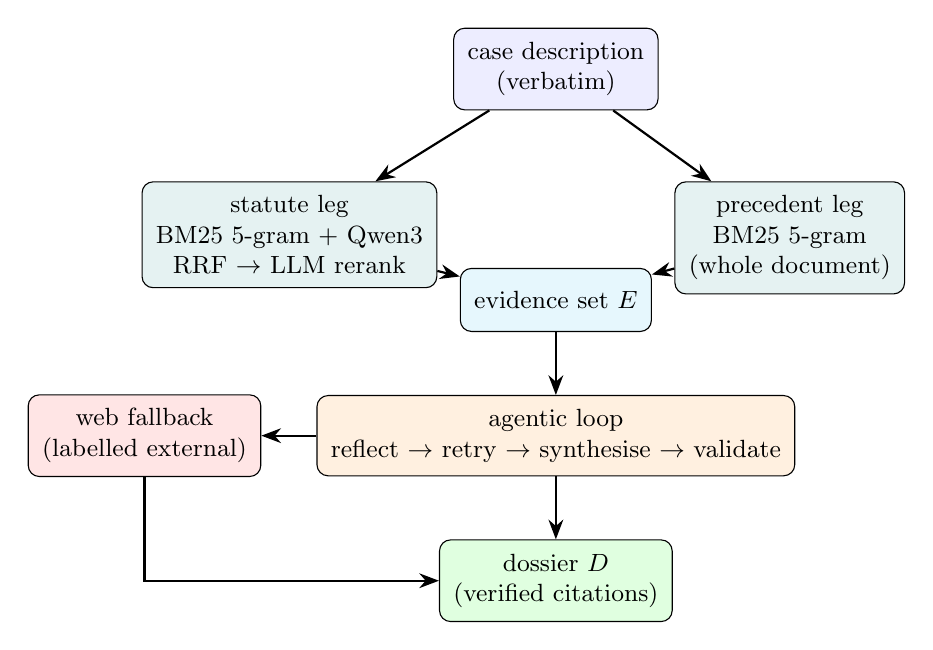
\begin{tikzpicture}[
  font=\small,
  box/.style={draw, rounded corners, align=center, inner sep=5pt,
              minimum height=8mm},
  layer/.style={draw, dashed, inner sep=6pt},
  arr/.style={-{Stealth[length=2.5mm]}, thick}]
\node[box, fill=blue!7] (q) {case description\\(verbatim)};
\node[box, fill=teal!10, below left=9mm and 2mm of q] (sleg)
  {statute leg\\BM25 5-gram + Qwen3\\RRF $\rightarrow$ LLM rerank};
\node[box, fill=teal!10, below right=9mm and 2mm of q] (pleg)
  {precedent leg\\BM25 5-gram\\(whole document)};
\node[box, fill=cyan!10, below=20mm of q] (ev) {evidence set $E$};
\node[box, fill=orange!12, below=8mm of ev] (loop)
  {agentic loop\\reflect $\to$ retry $\to$ synthesise $\to$ validate};
\node[box, fill=green!12, below=8mm of loop] (d) {dossier $D$\\(verified citations)};
\node[box, fill=red!10, left=7mm of loop] (fb) {web fallback\\(labelled external)};

\draw[arr] (q) -- (sleg);
\draw[arr] (q) -- (pleg);
\draw[arr] (sleg) -- (ev);
\draw[arr] (pleg) -- (ev);
\draw[arr] (ev) -- (loop);
\draw[arr] (loop) -- (d);
\draw[arr] (loop) -- (fb);
\draw[arr] (fb.south) |- (d.west);
\end{tikzpicture}
\figcaption{System architecture. The evidence layer retrieves
through task-conditional legs; the control layer judges, recovers,
synthesises, and validates; the fallback produces labelled
external material only on persistent insufficiency.}
\label{fig:arch}
\end{center}

\section{The Retrieval Substrate}
\subsection{Document Representation}
Precedent documents extend to tens of thousands of tokens and are
indexed whole where the lexical leg requires document-spanning
phrase context, and by recursive splitting at a 512-token window
with 50-token overlap where chunk-level retrieval is configured;
Chapter 3 showed the choice to be second-order for BM25.
Expanded-corpus statutes arrive already segmented at section
boundaries. Each chunk records its parent document identifier,
and retrieval deduplicates chunk hits to document hits so that
evidence is always reported at document granularity.

\subsection{The Lexical Leg}
The lexical leg indexes documents as word $n$-grams under BM25S
with $k_1=1.6$, $b=0.7$. Statutory and precedential language is
phrasal, and phrase matching is the source of this leg's
strength: on precedent retrieval the 5-gram variant is the
strongest non-fine-tuned configuration measured by any mechanism
in this study. The leg is deterministic, auditable, and
cache-addressed.

\subsection{The Dense Leg}
The dense leg embeds chunks with an instruction-prompted
bi-encoder and retrieves by inner product over normalised
vectors. Corpus embeddings are cached to disk so encoding is a
one-time cost; per-query encoding adds sub-second latency. The
serving configuration employs the 0.6B Qwen3-Embedding variant.
We hypothesise that increasing model parameters and context
length improves retrieval performance, as demonstrated by the
gain from the 0.6B to the 4B variant in
Table~\ref{tab:firststage} and confirmed externally on BSARD,
where the 4B leg lifts R@100 from 51.65 to 67.67
(Table~\ref{tab:bsard}).

\subsection{Fusion and Reranking}
Where both legs operate, reciprocal rank fusion merges them at
$k=60$ over each leg's top ranks. On the statute leg the fused
pool is then reranked listwise: the twenty strongest candidates
are presented as numbered snippets and the model returns a
relevance ordering, with the fused order preserved unchanged upon
any failure. The precedent leg omits the dense component and the
reranker entirely.

\section{The Agentic Control Loop}
The controller is a bounded state machine over the evidence set
$E$: retrieve, reflect, optionally retry once, synthesise,
validate. Figure~\ref{fig:loop} shows the flow, and each state is
specified below.

\begin{center}
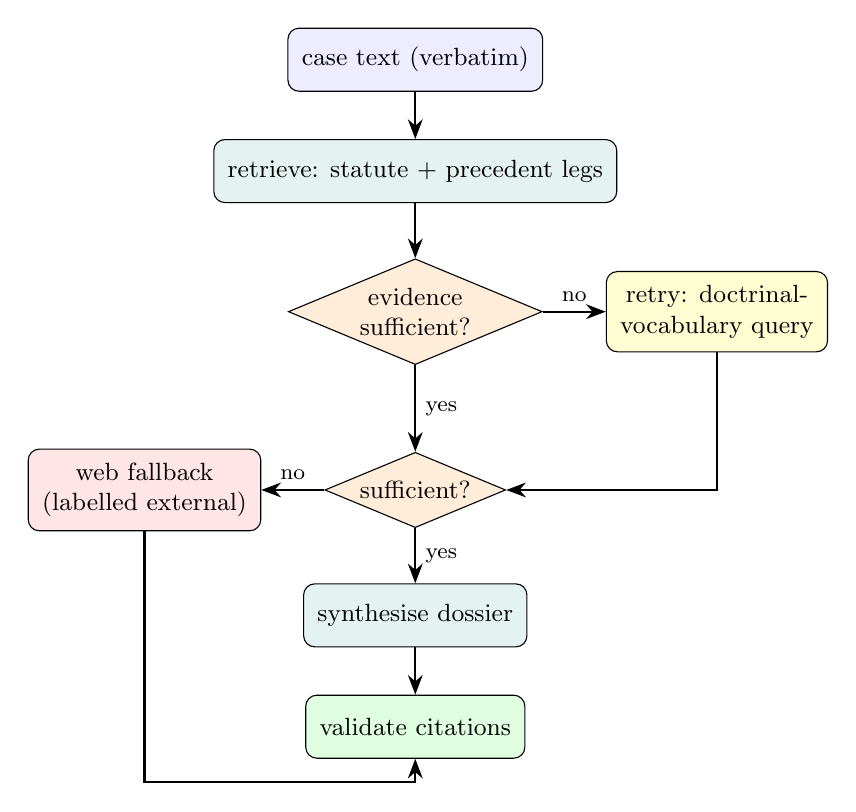
\begin{tikzpicture}[
  font=\small,
  box/.style={draw, rounded corners, align=center, inner sep=5pt,
              minimum height=8mm},
  dec/.style={draw, diamond, aspect=2.4, align=center,
              inner sep=1.5pt},
  arr/.style={-{Stealth[length=2.5mm]}, thick},
  lbl/.style={font=\footnotesize, midway, above}]
\node[box, fill=blue!7] (q)  {case text (verbatim)};
\node[box, fill=teal!10, below=6mm of q]  (r1) {retrieve: statute + precedent legs};
\node[dec, fill=orange!15, below=7mm of r1] (d1) {evidence\\sufficient?};
\node[box, fill=yellow!18, right=8mm of d1] (r2) {retry: doctrinal-\\vocabulary query};
\node[dec, fill=orange!15, below=11mm of d1] (d2) {sufficient?};
\node[box, fill=teal!10, below=7mm of d2] (sy) {synthesise dossier};
\node[box, fill=green!12, below=6mm of sy] (va) {validate citations};
\node[box, fill=red!10, left=8mm of d2] (fb) {web fallback\\(labelled external)};

\draw[arr] (q) -- (r1);
\draw[arr] (r1) -- (d1);
\draw[arr] (d1) -- node[lbl]{no} (r2);
\draw[arr] (r2.south) |- (d2.east);
\draw[arr] (d1) -- node[lbl, right]{yes} (d2);
\draw[arr] (d2) -- node[lbl]{no} (fb);
\draw[arr] (d2) -- node[lbl, right]{yes} (sy);
\draw[arr] (sy) -- (va);
\draw[arr] (fb.south) |- ($(va.south)+(0,-3mm)$) -| (va.south);
\end{tikzpicture}
\figcaption{The agentic loop. Reflection judges evidence
semantically on every query; a single reformulated retry executes
upon a negative verdict; residual gaps route to a labelled
external fallback.}
\label{fig:loop}
\end{center}

\begin{description}
\item[Retrieve.] The case text is issued verbatim to both legs.
  Chapter 3 establishes that every alternative loses.
\item[Reflect.] The language model examines the evidence and
  determines whether it genuinely addresses the case. The
  judgment is semantic rather than score-based, because a lexical
  score cannot distinguish the correct statute from a similarly
  named incorrect one: sections of the Bharatiya Nyaya Sanhita,
  the Bharatiya Nagarik Suraksha Sanhita, and the Bharatiya
  Sakshya Adhiniyam share much of their vocabulary and score
  comparably while only one is germane. Upon a negative verdict
  the model additionally formulates refined queries in doctrinal
  vocabulary, the phrasing statutory text itself employs, because
  bare section numbers do not occur in section bodies.
\item[Retry.] A negative verdict triggers one further retrieval
  round using the refined queries, and the merged evidence is
  judged once more. The loop is bounded at a single retry, since
  a lexical retriever that has failed twice rarely surfaces new
  material on a third attempt.
\item[Synthesise.] The model produces a structured dossier from
  the final evidence: a direct answer, the applicable provisions,
  a grounded analysis, and recommended steps. The prompt requires
  the answer to state what the cited provisions establish and
  prohibits commentary about unused or absent documents; where
  the evidence cannot support an answer, the dossier states so
  once rather than fabricating authority.
\item[Validate.] Every citation in the dossier is intersected
  with the retrieved set, and unverifiable identifiers are
  discarded with a warning. The check is mechanical and admits no
  exceptions.
\item[Fallback.] If the post-retry verdict remains negative, the
  residual gap is answered through web search, and the result is
  labelled as not corpus-grounded. External material may inform
  the answer; it is never presented as retrieved authority.
\end{description}

\begin{center}
\begin{minipage}{5.1in}
\noindent\textbf{Algorithm 1\quad Agentic control loop}\\[1mm]
\hrule\vspace{1.5mm}
\begin{algorithmic}[1]
\Require case description $q$
\State $E \gets$ \Call{Retrieve}{$q$} \Comment{verbatim to both legs}
\State $v \gets$ \Call{Reflect}{$q, E$} \Comment{semantic verdict}
\If{$v = \mathrm{insufficient}$}
    \State $q' \gets$ \Call{Reformulate}{$q, E$} \Comment{doctrinal vocabulary}
    \State $E \gets E \cup\; $\Call{Retrieve}{$q'$} \Comment{bounded retry}
    \State $v \gets$ \Call{Reflect}{$q, E$}
\EndIf
\If{$v = \mathrm{insufficient}$}
    \State $F \gets$ \Call{WebFallback}{$q$} \Comment{labelled external}
\Else
    \State $F \gets \emptyset$
\EndIf
\State $D \gets$ \Call{Synthesise}{$q, E \cup F$}
\State \Call{Validate}{$D, E$} \Comment{discard unverifiable citations}
\State \Return $D$
\end{algorithmic}
\vspace{1mm}
\hrule
\end{minipage}
\end{center}

\section{Expanded Statutory Corpus}
The benchmark statute collection is bounded by design; real
queries invoke legislation it does not contain, including the
2023 criminal codes, the Digital Personal Data Protection Act,
the Indian Easements Act, and the Insolvency and Bankruptcy Code.
The statute leg is therefore extended with a corpus assembled
from two public sources: a collection of Indian central acts in
India Code markdown~\cite{indianlegalacts} and the KanoonGPT
legal documents corpus~\cite{kanoongpt}. Approximately 300
central statutes were selected across criminal, civil and
property, family, consumer, finance and insolvency, labour,
environment, health, governance, intellectual property, and
digital regulation. Each act is segmented at section markers into
one document per section, and the act title is prepended to each
section's indexed text. This last detail is load-bearing: section
bodies never contain their act's name, so an act-name query
cannot lexically distinguish the Bharatiya Nyaya Sanhita from the
similarly named procedural and evidence codes unless the title is
indexed. Candidate source texts are scored by English legal-term
density to reject corrupted encodings.

\begin{center}
\tabcaption{Composition of the expanded statute index. The
precedent leg retains its 3,183 IL-PCSR documents.}
\label{tab:corpus}
\vspace{2mm}
\begin{tabular}{lr}
\toprule
Corpus segment & Section documents \\
\midrule
Criminal codes and procedure & 1,027 \\
Finance, insolvency, securities, taxation & 3,307 \\
Civil procedure, property, succession & 2,556 \\
Labour codes and industrial law & 1,571 \\
Family and personal law & 1,224 \\
Health, food, mental healthcare & 2,318 \\
Environment, forests, energy & 1,204 \\
Consumer, competition, commerce & 1,087 \\
Governance, transparency, public services & 1,612 \\
Digital regulation (IT Act, DPDP, telecom) & 517 \\
Intellectual property & 1,296 \\
Constitutional and administrative law & 1,846 \\
Other central acts & 9,573 \\
\midrule
Expanded corpus (302 acts) & 27,138 \\
IL-PCSR statutes (retained) & 936 \\
\midrule
Indexed statute leg & 28,074 \\
\bottomrule
\end{tabular}
\end{center}

\chapter{Implementation and Application Development}

\section{Technology Stack}
The framework is implemented in Python. Retrieval uses BM25S for
the lexical legs~\cite{bm25s}, sentence-transformers for dense
encoding, and NumPy matrix products for similarity search; the
agent and reranker call an externally hosted language model
through a plain HTTP provider layer. The experiment harness and
the server share the same loader, chunker, retriever classes, and
evaluation code, which keeps the served pipeline identical to the
benchmarked one. Heavy computation is offloaded: dense corpus
encoding ran on a Kaggle T4 and a Modal A10G GPU, while the
serving machine only loads the cached embedding matrix. The
server is a FastAPI application; the demonstration interface is a
React single-page application.

\section{The Evaluation Harness}
The harness is configuration-driven. Each experiment is a JSON
specification naming its chunking strategy, retriever, query
strategy, and reranker; the runner indexes once per corpus
(content-addressed, so an index is rebuilt only when corpus bytes
change), issues all 627 queries through one code path, and writes
both an aggregate summary and a per-query record containing the
run's git commit, config hash, seed, and platform.

\section{The Agent Implementation}
The controller is implemented as a single orchestrator class with
explicit steps. The retrieval step merges hits per task into an
evidence map keyed by document identifier, keeping the best score
per document across rounds. The reflection step presents the top
evidence identifiers and titles to the model and parses a JSON
verdict; unparseable or failed verdicts fail open as sufficient,
so an LLM outage cannot mark good evidence insufficient. The
synthesis step assembles the top-$k$ evidence snippets with their
identifiers and titles into the prompt and parses the returned
JSON dossier. The validation step intersects the dossier's
citation identifiers with the evidence map and drops any that do
not occur there. Each step records its inputs and latency into a
trace that the application renders, so every agent decision is
inspectable.

\section{The Serving Application}
The server exposes three analysis modes that differ honestly in
what they run. \emph{Single-shot} issues the case text to both
first-stage legs and returns raw evidence with no LLM call, which
makes it the free baseline and the retrieval inspection view.
\emph{Agent-synthesis} runs the recommended configuration:
verbatim retrieval, then grounded dossier generation with
citation validation. \emph{Agent-full} executes the complete
loop: retrieve, reflect, bounded retry, synthesise, validate, and
a labelled web fallback on persistent insufficiency. The statute
leg is assembled at startup as the measured configuration
permits: lexical retrieval alone when no dense embedding cache is
present, RRF fusion when the cache exists, and listwise reranking
on the agent paths when an LLM key is configured. Each response
carries the leg labels actually used, so the interface cannot
misrepresent the active pipeline. Conversations persist to a
server-side store with search, pin, rename, and delete
operations, and each analysis is deep-linkable by identifier.

The interface renders the dossier first, then the underlying
evidence as inspectable cards: each source carries its corpus,
retrieval score, and a query-relevant excerpt chosen by
content-term overlap with the case text, so the grounding of
every answer is verified by inspection rather than asserted.
External fallback material appears in a separately labelled
section.

\section{End-to-End Request Flow}
A case description enters the API; the server issues it verbatim
to both legs. The statute leg retrieves through its fused,
reranked pipeline; the precedent leg retrieves through lexical
matching alone. The merged evidence set passes to reflection; on
a sufficiency verdict, synthesis produces the dossier directly;
on insufficiency, refined queries re-retrieve once, and a
persistent failure routes the residual question to the labelled
web fallback. Citation validation then filters the dossier before
the response is stored and rendered. The full trace, including
query counts, verdicts, and per-step latency, is returned with
the answer.

\chapter{Results, Evaluation, and Discussion}

\section{Evaluation Framework}
Three layers of evidence are kept distinct throughout this
chapter: benchmark retrieval metrics (Chapter 3), agent
behavioural statistics on the 50-query slice, and live
verifications on the served system over the expanded corpus.
Conflating them would produce claims the data does not support.

\section{System-Level Behaviour}
Table~\ref{tab:sys} summarises the assembled system as measured.

\begin{center}
\small
\tabcaption{The assembled system as measured. Retrieval rows are
development-split; the test row is the test-split BM25 run.}
\label{tab:sys}
\vspace{2mm}
\begin{tabular}{p{0.34\linewidth}p{0.58\linewidth}}
\toprule
Property & Measured value \\
\midrule
Statute leg (dev) & RRF 5-gram + Qwen3: F1@10 14.68, MAP 19.12,
MRR 40.53; + LLM rerank: F1@10 14.83, MAP 25.20, MRR 50.88 \\
Precedent leg (dev) & 5-gram BM25: F1@10 20.73, MAP 39.90,
MRR 57.28 \\
Test-split BM25 rec-512 & F1@10 12.92 LSR / 17.92 PCR \\
Agent loop (50 q) & 78 retrieve calls; 22/50 sufficient at first
verdict; 49/50 dossiers; 167/167 citations valid \\
Indexed corpora & 28,074 statute docs; 3,183 precedent docs \\
\bottomrule
\end{tabular}
\end{center}

\section{Live Verifications}
Five queries exercised against the served system illustrate the
loop's operating modes.

\begin{livebox}{Statute query: punishment for murder}{blue}
\textbf{Query.} What is the punishment prescribed for murder
under the Bharatiya Nyaya Sanhita, 2023?\\
\textbf{Retrieved.} BNS \S\S\,103, 104, 105; IPC \S\,302
(predecessor provision).\\
\textbf{Loop.} Evidence judged sufficient on the first pass; no
retry.\\
\textbf{Answer.} ``Section 103(1) of the Bharatiya Nyaya
Sanhita, 2023 provides that whoever commits murder shall be
punished with death or imprisonment for life and shall also be
liable to fine. Under section 103(2), each member of a group of
five or more acting in concert to commit murder \ldots''
\end{livebox}

\begin{livebox}{Case-law query: unlawful eviction}{teal}
\textbf{Query.} A landlord forcibly evicted a tenant without
notice and locked the premises; the tenant seeks relief for
unlawful eviction and recovery of possession.\\
\textbf{Retrieved.} Specific Relief Act 1963 \S\,6; Delhi Rent
Control Act 1958 \S\S\,14, 19, 22; four precedents.\\
\textbf{Loop.} First verdict insufficient; doctrinal retry.\\
\textbf{Answer.} ``\ldots a person dispossessed without consent
and otherwise than in due course of law may bring a suit
concerning that dispossession, and \ldots a person entitled to
possession may seek recovery through the civil procedure
provided by law.''
\end{livebox}

\begin{livebox}{General legal knowledge: culpable homicide and
murder}{violet}
\textbf{Query.} What is the difference between culpable homicide
and murder under Indian criminal law?\\
\textbf{Retrieved.} IPC \S\S\,299, 300; BNS \S\S\,100, 101.\\
\textbf{Loop.} First verdict insufficient; doctrinal retry.\\
\textbf{Answer.} ``Culpable homicide is the broader offence.
Under Sections 299 IPC and 100 BNS, it is established where a
person causes death with the specified intention or knowledge.
Murder is the more serious, narrower category: under Sections
300 IPC and 101 BNS \ldots''
\end{livebox}

\begin{livebox}{Out-of-corpus: an international obligation}{orange}
\textbf{Query.} What obligations does India bear under the
Vienna Convention on Consular Relations for detained foreign
nationals?\\
\textbf{Retrieved.} BNSS \S\,48; Immigration and Foreigners Act
2025; Extradition Act 1962; Foreigners Act 1946.\\
\textbf{Loop.} Insufficient, retried, then answered only from
domestic provisions; the convention text is absent from the
corpus, and no external material was presented as retrieved
authority.\\
\textbf{Answer.} ``The cited provisions establish domestic
procedural duties upon arrest: officers must promptly notify a
person nominated by the arrested individual, record whom they
informed, and the Magistrate must check compliance \ldots''
\end{livebox}

\begin{livebox}{Out-of-scope query: integrity check}{gray}
\textbf{Query.} Explain how Dijkstra's shortest-path algorithm
works on a weighted graph.\\
\textbf{Retrieved.} Off-topic municipal and railway provisions;
the corpus contains no relevant material.\\
\textbf{Loop.} Insufficient on both rounds.\\
\textbf{Answer.} ``The evidence does not establish an answer.''
The loop declined to fabricate one.
\end{livebox}

The first box exhibits the clean path: sufficient evidence on the
first pass, a corpus-grounded answer, no recovery. The second
and third show the loop's characteristic behaviour: a retrieval
failure invisible to lexical scores was caught by the semantic
verdict, and the doctrinal retry completed the correction inside
the corpus, drawing on the expanded statute collection for the
Delhi Rent Control provisions. The fourth box marks the corpus
boundary honestly: the answer confines itself to the domestic
provisions retrieved, and the missing convention text is neither
invented nor passed off. The fifth states the property a legal
tool cannot compromise: confronted with a query the corpus
cannot answer, the system says so rather than synthesising
authority that does not exist.

\section{Interpretation}
Four properties of the results deserve explicit discussion.

First, retrieval quality and answer reliability are different
quantities, and the system optimises them in different places.
The retrieval chapter maximises ranking metrics; the agent loop
then guards the property metrics cannot express: whether the
evidence actually answers the question and whether every citation
is real. The 28 negative first verdicts in the agent benchmark
are the loop working as designed, not a defect rate.

Second, the asymmetric architecture is not a compromise but the
measured optimum. A uniform pipeline would either give statutes a
lexical leg twenty MAP points below its dense alternative, or
give precedents a fused leg that dilutes the strongest
non-fine-tuned configuration in the study.

Third, the agent's contribution is located where the measurements
place it. The router arm of the agent benchmark shows that
LLM-written retrieval queries lose nearly twenty MAP points on
the lexical task; what the LLM contributes is judgment,
recovery, synthesis, and citation discipline, and the
architecture confines it to exactly those functions.

Fourth, the negative results are load-bearing. The study can
state with evidence, rather than with intuition, that long legal
queries must be issued verbatim, that bounded-context rerankers
must not be used on them, and that fusion must be conditioned on
leg quality. These rules generalise beyond the specific
configuration measured.

\section{Limitations and Threats to Validity}
Development-split metrics at fixed depth are reported alongside,
not equated with, the published test-split best-$k$ rows; a
same-protocol evaluation of the assembled configuration on the
test split remains outstanding, and the single test-split run
performed covers lexical retrieval only. The 4B embedder that
marks the measured quality ceiling requires GPU inference; the
serving configuration employs the 0.6B variant and accepts the
corresponding gap. Queries to dense models were truncated at
2,048 tokens, so the dense legs were measured on roughly half the
average case description; the results favour them nonetheless.
The dense legs evaluated on the precedent task used chunked
indexes, while the champion precedent row used a whole-document
index, a pairing fixed by $n$-gram tokenisation cost rather than
by choice. Precedent coverage is bounded by the benchmark's
3,183 documents, and queries beyond it rely on the labelled
fallback. The retry is bounded at one round by design; a learned
stopping criterion could recover a small residue of failures.
Finally, the agent benchmark is 50 queries on one model
configuration; the behavioural findings are consistent but their
generality across models is unmeasured.

\chapter{Conclusion and Future Work}

\section{Conclusion}
This dissertation set out to determine which pipeline a
verifiable legal-analysis system should run, and the measurements
answered the question consistently. The two retrieval tasks are
distinct problems warranting distinct machinery: phrase-level
lexical retrieval for precedents, long-context dense retrieval
with fusion and listwise reranking for statutes. Long case
descriptions must reach the retriever verbatim; every substitute
tested lost ground. A reranker is warranted only where the
relevance signal is semantic and only when it can read the input.
An agentic loop earns its place through the guarantees it adds,
namely evidence-sufficiency judgment, a bounded retry, a labelled
fallback, and universally validated citations, rather than
through retrieval planning. A first external validation on the
French BSARD benchmark and the Indian AILA benchmark confirms
that these design rules travel: on BSARD the pipeline exceeds
every published zero-shot baseline without modification or
retraining, the 4B dense leg alone closes most of the remaining
gap to the fine-tuned ceiling, and on AILA the same
task-conditional asymmetry and the fusion-complementarity rule
replicate unchanged. The
expanded corpus and the demonstration application render the
measured pipeline a functioning system that answers queries the
benchmark itself cannot, including the 2023 criminal codes.

\section{Findings in Relation to the Research Objectives}
The first two objectives are met by the experimental programme:
Tables~\ref{tab:firststage} and \ref{tab:fusion} establish which
retrieval, fusion, and reranking mechanisms are effective for
each corpus, and Table~\ref{tab:find2arch} records how those
measurements, including the uniformly negative query-processing
results of Table~\ref{tab:query}, determined the derived
architecture. The third objective is met by the agent benchmark:
the bounded loop contributed sufficiency judgment, one-shot
recovery, and citation integrity, with all 167 emitted citations
valid. The fourth is met by the live verifications: the expanded
corpus resolves queries on legislation the benchmark does not
contain. The fifth objective, transfer to other legal datasets
and jurisdictions, receives its first empirical test in
Section~3.13: the assembled legs outperform every published
zero-shot baseline on the French BSARD benchmark, and on the
Indian AILA benchmark the same lexical-precedent and
semantic-statute asymmetry and the fusion-complementarity rule
replicate, in both cases without modification or retraining.
Broader transfer across further corpora remains open.

\section{Future Work}
A same-protocol test-split evaluation of the assembled
configuration would convert the protocol-aware comparison into a
direct numerical one, and is the first outstanding item.
Fine-tuning the dense leg on the 5,017 training queries
constitutes the largest unclaimed improvement, since the
published fine-tuned rows indicate the headroom supervision
provides; a contrastive fine-tune of Qwen3-0.6B is configured but
not yet evaluated. A task-aware precedent reranking prompt, a
learning-to-rank fusion trained on per-leg features, and
cross-task conditioned retrieval are all specified extensions the
harness supports directly. On the corpus side, state-level
legislation, municipal bye-laws, and state police acts are the
next class of statutes real queries invoke, and the ingestion
pipeline requires no modification to accept them. On the agent
side, a learned sufficiency threshold, a second bounded retry,
and a numeric groundedness score per dossier are natural
strengthenings. Finally, the fifth objective stands partially
open in empirical terms: Section~3.13 supplies the first
cross-corpus evidence, on French statutory text and on a second
Indian benchmark, and extending
the same battery to the case-law and non-European benchmarks the
literature supplies, the COLIEE Canadian case-law
collection~\cite{rabelo2022coliee21} and the Chinese
case-retrieval corpora LeCaRD~\cite{ma2021lecard} and
CAIL~\cite{xiao2018cail2018}, is the outstanding test. The
evaluation itself can be
deepened: a human study of dossier correctness against expert
legal judgment would measure the property the citation validator
can only approximate.

\bibliographystyle{unsrtnat}
\bibliography{references}

\end{document}
